\documentclass[conference]{IEEEtran}
\IEEEoverridecommandlockouts

\usepackage{cite}
\usepackage{amsmath,amssymb,amsfonts}
\usepackage{graphicx}
\usepackage{booktabs}
\usepackage{textcomp}
\usepackage{xcolor}
\usepackage{array}
\usepackage[spanish]{babel}
\usepackage[utf8]{inputenc}
\usepackage{hyperref}
\usepackage{float}

\def\BibTeX{{\rm B\kern-.05em{\sc i\kern-.025em b}\kern-.08em
    T\kern-.1667em\lower.7ex\hbox{E}\kern-.125emX}}

\begin{document}

\title{Análisis de Readmisiones Hospitalarias, Recurrencia y Duración de Estancia en Pacientes Diabéticos\\
\large Proyecto Final --- Analítica de Datos}

\author{\IEEEauthorblockN{Hector Raul Becerril Villamil, Elena Carolina Sánchez Araiza}
\IEEEauthorblockA{\textit{Universidad Iberoamericana, Ciudad de México} \\
\textit{Prof. Rodrigo Cárdenas Domínguez} \\
Primavera 2026}
}

\maketitle

\begin{abstract}
Este trabajo modela tres fenómenos clínico-operativos del dataset \textit{Diabetes 130-Hospitals}: la readmisión hospitalaria dentro de los 30 días, la recurrencia de ingresos previos y la duración de la estancia. Tras una limpieza agresiva --- eliminación de columnas con $>$95\% de faltantes, reducción a un registro por paciente y exclusión de pacientes fallecidos u hospitalarios terminales --- se trabajó con 69\,970 observaciones. Un análisis exploratorio detectó asimetría marcada en la estancia (skew $\approx 1.18$) y sobredispersión en el número de ingresos (var/media $\approx 2.05$), lo que orientó la elección de modelos. Una regresión logística obtuvo un AUC de 0.608 sobre el conjunto de prueba, identificando al historial de admisiones previas como el predictor modificable más fuerte (OR $\approx 1.40$ por ingreso adicional). El modelo binomial negativo superó claramente al Poisson ($\Delta$AIC $\approx 8\,500$), confirmando la sobredispersión. La regresión Gamma con enlace logarítmico ajustó de manera razonable a la estancia (pseudo $R^2 \approx 0.28$). Los hallazgos se traducen en recomendaciones concretas para la directiva del hospital: priorizar un programa de transición de cuidados enfocado en pacientes con uso previo de urgencias e ingresos repetidos.
\end{abstract}

\begin{IEEEkeywords}
readmisiones hospitalarias, diabetes, regresión logística, binomial negativa, Gamma GLM, EDA
\end{IEEEkeywords}

\section{Introducción}
La readmisión temprana en pacientes con diabetes mellitus no es solo un problema clínico --- es un tema financiero. En EE.UU., los Centers for Medicare \& Medicaid Services imponen reducciones al reembolso cuando un hospital excede ciertos umbrales de reingreso a 30 días \cite{cms_hrrp}. Para un hospital grande, esto se traduce en millones de dólares al año. Y en salud, como en tantas cosas, lo que no se mide no se gestiona.

Nos pidieron desde la dirección del hospital responder tres preguntas que suenan sencillas pero que no lo son: ¿quiénes son los pacientes con más riesgo de volver pronto?, ¿por qué algunos ingresan tan seguido?, ¿qué hace que unas estancias se alarguen más que otras? La primera se ataca con clasificación binaria; la segunda es un problema de conteo; la tercera, de regresión sobre una variable continua y sesgada. Cada uno exige una herramienta distinta, y eso es parte de lo que hace al proyecto interesante.

El resto del documento sigue el orden natural del trabajo: datos y preparación (§II), análisis exploratorio (§III), inferencia (§IV), los tres modelos (§V) y, al final, las conclusiones accionables que terminaron en la presentación ejecutiva (§VI).

\section{Datos y Preparación}
El conjunto \textit{Diabetes 130-Hospitals} agrupa 101\,766 admisiones entre 1999 y 2008 de 130 hospitales de EE.UU. \cite{strack2014}. Son 50 variables que mezclan datos demográficos, indicadores clínicos y 23 fármacos.

\subsection{Calidad del dato}
Revisar faltantes fue el primer paso obligado. Tres columnas saltaban a la vista: \texttt{weight} con 96.9\% de vacíos, \texttt{medical\_specialty} con 49.1\% y \texttt{payer\_code} con 39.6\%. A \texttt{weight} la descartamos sin pensarlo demasiado --- con esa proporción, cualquier imputación sería fabricación pura. Las otras dos se conservaron con la categoría \textit{Desconocido}, que al menos captura la posibilidad (nada despreciable) de que el hecho mismo de no registrar la especialidad esté correlacionado con algún patrón.

\subsection{Independencia de observaciones}
Un detalle que casi se me pasa: \texttt{patient\_nbr} se repite cada vez que un mismo paciente regresa. Si dejo todas las admisiones como filas independientes, rompo un supuesto clave de casi cualquier prueba estadística --- las observaciones dejan de ser i.i.d. La solución rápida fue quedarnos con el primer encuentro de cada paciente. Menos datos, pero datos honestos.

Después filtramos egresos terminales (códigos 11, 13, 14, 19, 20, 21 del mapeo de disposición), porque esos pacientes no tienen forma de ser readmitidos y sólo inflan artificialmente el denominador. Tras todo el proceso quedaron 69\,970 observaciones.

\subsection{Transformaciones}
La edad venía en rangos (\texttt{[60-70)}) --- la reemplazamos por su punto medio para poder usarla como numérica. Los diagnósticos principales \texttt{diag\_1} con su catálogo ICD-9 completo eran demasiado granulares (más de 700 códigos distintos), así que los agrupamos en nueve bloques clínicos estándar siguiendo la taxonomía del AHRQ \cite{ahrq_ccs}: circulatorio, respiratorio, digestivo, diabetes, lesiones, musculoesquelético, genitourinario, neoplasmas y otros. La variable objetivo \texttt{readmitted} se binarizó: 1 si el paciente regresó en $<$30 días, 0 en los otros dos casos (\texttt{>30} y \texttt{NO}).

Creamos además dos variables derivadas útiles: \texttt{uso\_medicacion\_diab} (binaria, indica si el paciente recibe medicamento para diabetes) y \texttt{cambio\_med} (binaria, indica si hubo cambio en la medicación durante la estancia). Ambas apuntan a la complejidad y severidad del caso, que luego resultarían predictores importantes.

\section{Análisis Exploratorio}
\begin{figure}[H]
\centering
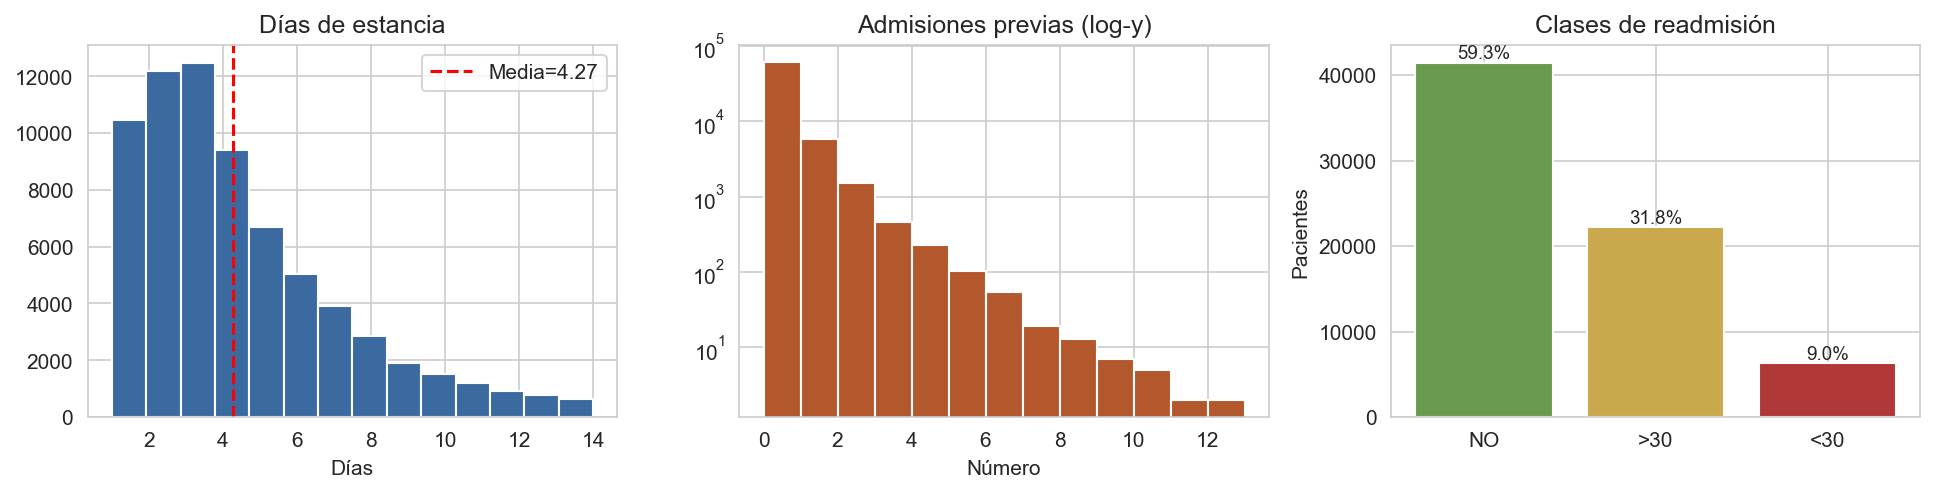
\includegraphics[width=0.95\linewidth]{figuras/fig1_distribuciones.png}
\caption{Distribuciones de las tres variables respuesta. La estancia es asimétrica a la derecha; las admisiones previas tienen una cola larguísima (nótese la escala log); la readmisión a 30 días ocurre en un 8.97\% de los casos.}
\label{fig:dist}
\end{figure}

Las tres distribuciones cuentan historias diferentes. La estancia se concentra entre 2 y 5 días pero con una cola que llega a 14; \texttt{number\_inpatient} tiene moda en cero y un puñado de pacientes con hasta 21 ingresos previos; y la tasa base de readmisión a 30 días es del 8.97\%, lo que ya avisa de un problema de desbalance de clases.

El EDA bivariado (Fig.~\ref{fig:box}) mostró que los pacientes readmitidos dentro de 30 días tienen, en mediana, un día más de estancia (4 vs 3) y reciben más medicamentos. La tabla~\ref{tab:readdiag} condensa el cruce con la categoría diagnóstica.

\begin{figure}[H]
\centering
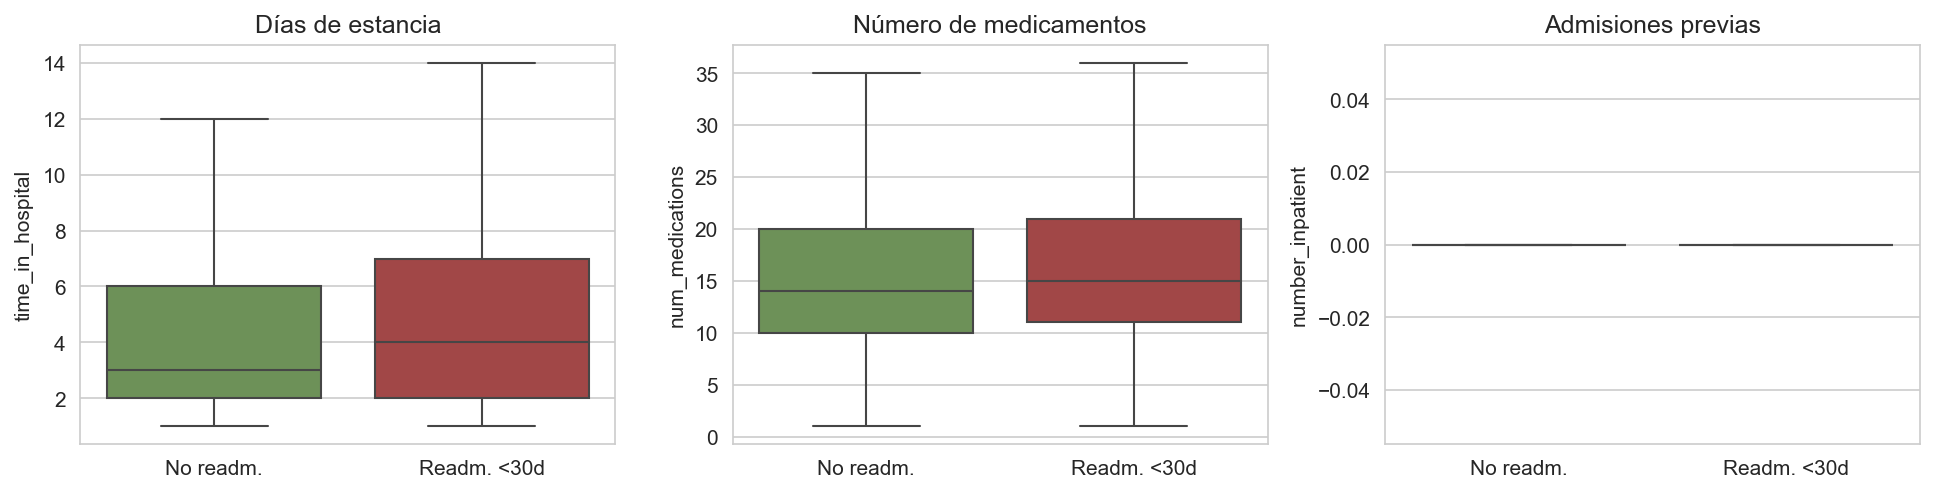
\includegraphics[width=0.95\linewidth]{figuras/fig2_boxplots_readmit.png}
\caption{Boxplots comparando pacientes no readmitidos vs. readmitidos en tres variables clínicas clave.}
\label{fig:box}
\end{figure}

Para mapear qué variables van juntas, calculamos la matriz de correlación de Spearman (Fig.~\ref{fig:corr}). Usamos Spearman y no Pearson porque ninguna de las variables es simétrica y Spearman sí captura relaciones monótonas no-lineales. Lo que salta a la vista es un clúster fuerte entre los conteos de utilización (\texttt{number\_inpatient}, \texttt{number\_emergency}, \texttt{number\_outpatient}): los pacientes que pisan el hospital pisan todo. También hay una correlación moderada entre \texttt{num\_medications}, \texttt{num\_lab\_procedures} y \texttt{time\_in\_hospital} --- cuanto más complejo el caso, más pruebas, más fármacos, más días. La correlación de la variable objetivo \texttt{readmit\_30d} con el resto es baja (máximo $\approx 0.11$ con \texttt{number\_inpatient}), lo que ya nos adelanta que un modelo lineal simple no dará AUC altísimo.

\begin{figure}[H]
\centering
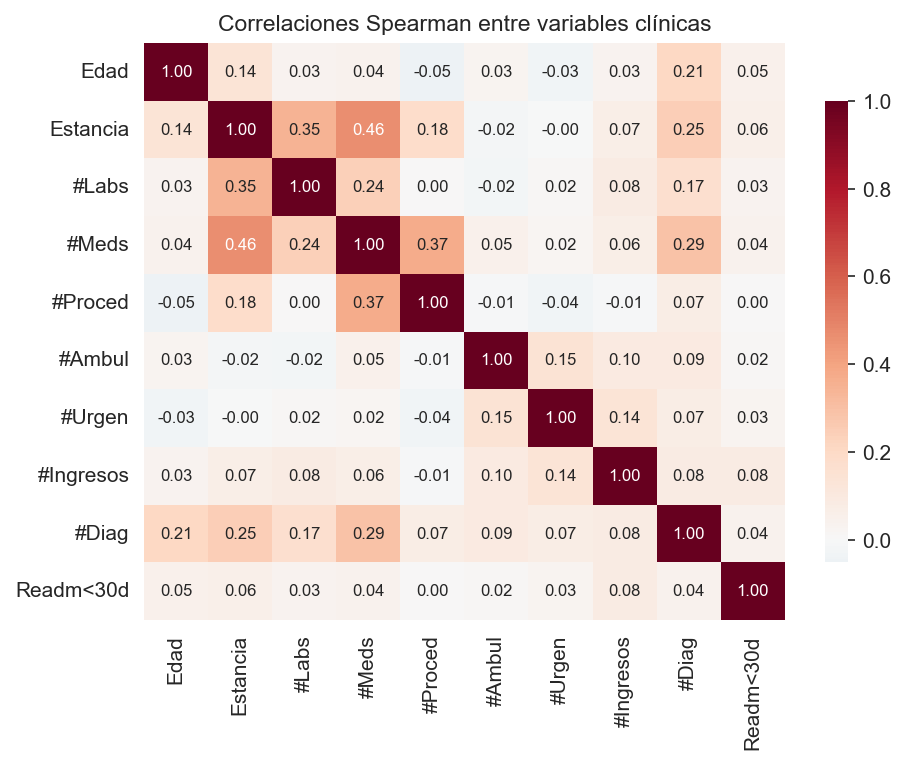
\includegraphics[width=0.85\linewidth]{figuras/fig6_corr_spearman.png}
\caption{Matriz de correlación de Spearman entre variables clínicas y la variable objetivo.}
\label{fig:corr}
\end{figure}

Un corte adicional: la tasa de readmisión cambia de forma no monótona con la edad (Fig.~\ref{fig:edad}). Los pacientes muy jóvenes casi no se reingresan --- aunque con muestras pequeñas---, y la tasa sube escalonadamente hasta estabilizarse entre 9 y 11\% en los grupos de 60 años en adelante. Eso tiene sentido clínico: los grupos etarios más altos acumulan comorbilidades que elevan el riesgo.

\begin{figure}[H]
\centering
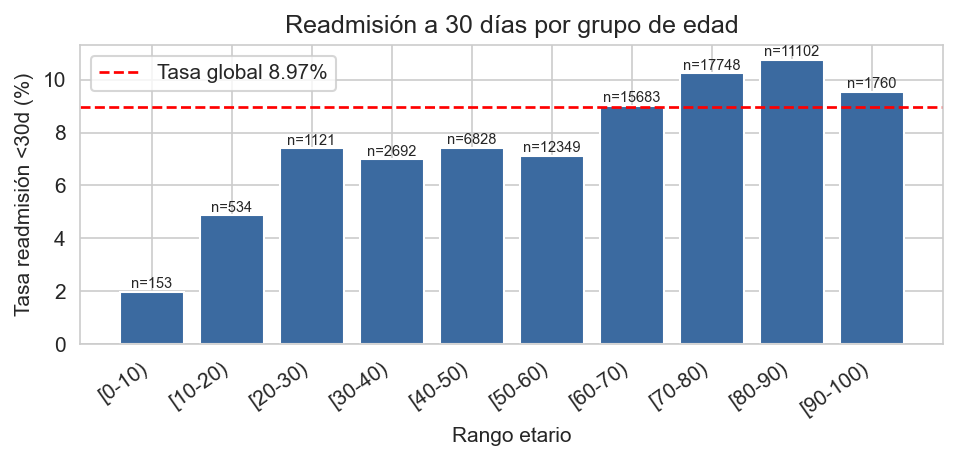
\includegraphics[width=0.92\linewidth]{figuras/fig7_readmit_edad.png}
\caption{Tasa de readmisión a 30 días por grupo etario. La línea roja marca la tasa global (8.97\%).}
\label{fig:edad}
\end{figure}

\begin{table}[H]
\caption{Tasa de readmisión a 30 días por categoría diagnóstica principal}
\label{tab:readdiag}
\centering
\begin{tabular}{lcc}
\toprule
\textbf{Categoría} & \textbf{Tasa readm. \%} & \textbf{n} \\
\midrule
Lesiones        & 10.78 & 2\,634 \\
Circulatorio    & 9.67  & 21\,081 \\
Diabetes        & 9.12  & 5\,498 \\
Genitourinario  & 8.98  & 3\,218 \\
Musculoesq.     & 8.39  & 4\,290 \\
Digestivo       & 8.02  & 6\,395 \\
Respiratorio    & 7.28  & 9\,384 \\
\bottomrule
\end{tabular}
\end{table}

\section{Inferencia Estadística}
Con $n = 4\,000$ muestras el test Shapiro-Wilk ya es inviable; usamos Kolmogorov-Smirnov. Para \texttt{time\_in\_hospital} estandarizada contra una normal obtuvimos $D = 0.179$, $p < 10^{-100}$ --- normalidad rotundamente rechazada. Contra una lognormal ajustada, $D = 0.107$: mejor, aunque sigue rechazando. Esto alineó la decisión de usar familia Gamma en el modelado.

Como las variables no son normales, comparamos grupos con pruebas no paramétricas:
\begin{itemize}
    \item \textbf{Mann-Whitney U} (estancia entre readmitidos y no): $U = 1.76\times 10^{8}$, $p = 1.7\times 10^{-56}$. Mediana: 3 días vs 4 días.
    \item \textbf{Chi-cuadrado} (categoría diagnóstica $\times$ readmit): $\chi^{2}=75.2$ con 9 g.l., $p = 1.45\times 10^{-12}$.
    \item \textbf{Kruskal-Wallis} (estancia entre grupos de edad): $H = 1\,438.97$, $p < 10^{-300}$.
\end{itemize}

Los $p$-valores son minúsculos, pero con $n > 60\,000$ casi cualquier diferencia sale significativa. Lo relevante aquí no es el \textit{p}, sino el tamaño del efecto --- una mediana adicional de un día de estancia, a escala hospitalaria, sí es operativamente relevante.

Checkpoint obligado antes de pasar al modelo de conteo: $\mathrm{Var}(\texttt{number\_inpatient})/\mathrm{E}[\texttt{number\_inpatient}] = 0.362/0.176 \approx 2.05$. Eso es sobredispersión clásica, así que Poisson pura no va a alcanzar.

\section{Modelado Estadístico}

\subsection{Modelo 1: Regresión logística para readmisión $<$30 días}
Ajustamos una regresión logística clásica con \texttt{statsmodels} sobre 75\% de los datos, estratificando por la clase. El modelo incluye 10 variables numéricas (edad, estancia, medicamentos, procedimientos, conteos de utilización y dos binarias: uso de medicación para diabetes y cambio en la medicación) más dummies para categoría diagnóstica y género.

\begin{figure}[H]
\centering
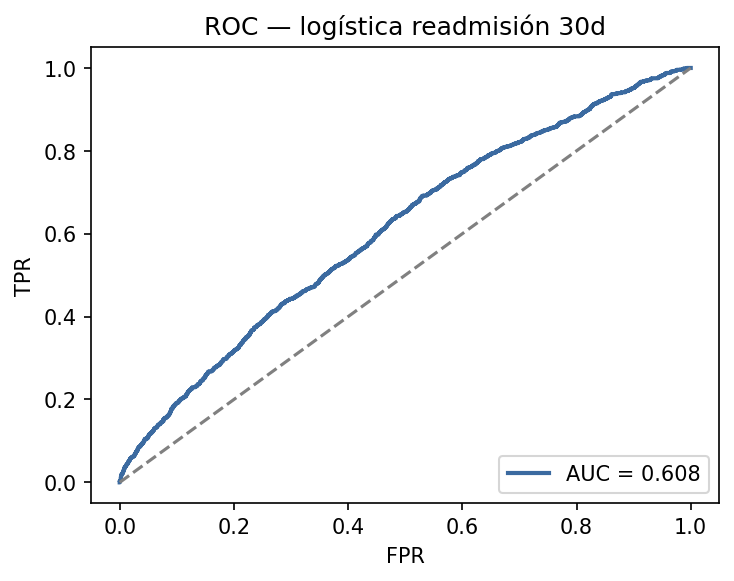
\includegraphics[width=0.75\linewidth]{figuras/fig3_roc_logistica.png}
\caption{Curva ROC del modelo logístico en el conjunto de prueba.}
\label{fig:roc}
\end{figure}

Desempeño en prueba: AUC $= 0.608$; pseudo $R^{2}$ de McFadden $= 0.023$. No es un gran clasificador, y conviene decirlo con honestidad: la readmisión temprana es un fenómeno notoriamente ruidoso y los estudios con datasets similares rara vez pasan del rango 0.60-0.65 sin incluir laboratorios detallados o notas clínicas \cite{rubin2018}.

Lo realmente útil está en los odds ratios (Tabla~\ref{tab:or}). Cada admisión previa adicional multiplica las odds de readmitirse por $\approx 1.40$; una visita adicional a urgencias en el año previo, por $\approx 1.07$; y los pacientes con medicación para diabetes tienen 1.21 veces las odds respecto a los que no. Estos tres son justamente los factores sobre los que un programa de transición de cuidados puede intervenir.

\begin{table}[H]
\caption{Odds ratios principales --- regresión logística}
\label{tab:or}
\centering
\begin{tabular}{lccc}
\toprule
\textbf{Variable} & \textbf{Coef.} & \textbf{OR} & \textbf{p-valor} \\
\midrule
\texttt{number\_inpatient}     & 0.340  & 1.405 & $<$0.001 \\
\texttt{uso\_medicacion\_diab} & 0.188  & 1.207 & $<$0.001 \\
\texttt{number\_emergency}     & 0.071  & 1.074 & $<$0.001 \\
\texttt{number\_diagnoses}     & 0.033  & 1.034 & $<$0.001 \\
\texttt{edad\_num}             & 0.005  & 1.005 & $<$0.01 \\
\bottomrule
\end{tabular}
\end{table}

\begin{figure}[H]
\centering
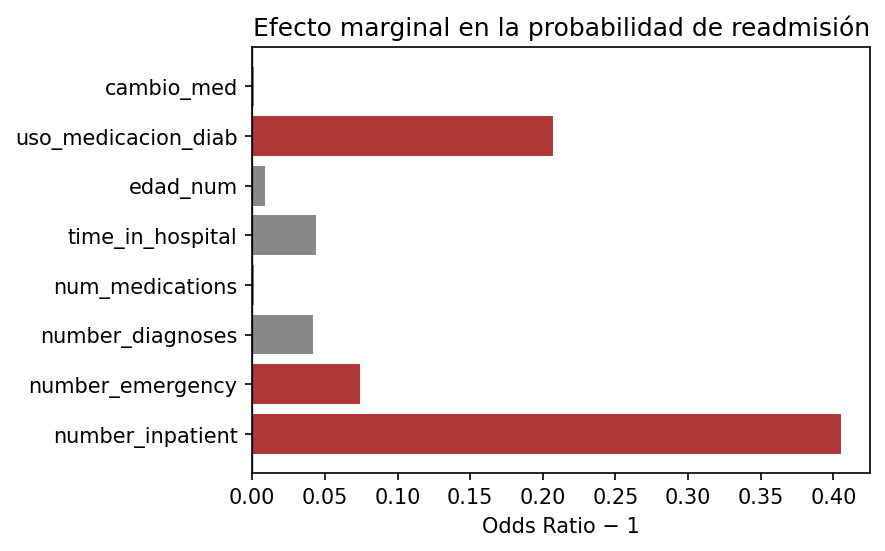
\includegraphics[width=0.95\linewidth]{figuras/fig4_or_logistica.png}
\caption{Efecto marginal (OR $- 1$) de las variables clínicas en la probabilidad de readmisión.}
\label{fig:or}
\end{figure}

\subsection{Modelo 2: Poisson vs. Binomial Negativa para recurrencia}
El primer ajuste fue Poisson. La dispersión Pearson resultó en 1.93, claramente por encima de 1 --- la sobredispersión del EDA se confirma en residuos. Estimamos $\alpha$ con el método auxiliar de Cameron-Trivedi: $\hat\alpha = 3.05$. Con ese valor se ajustó la binomial negativa. Resultado:

\begin{table}[H]
\caption{Comparación Poisson vs. Binomial Negativa}
\label{tab:nb}
\centering
\begin{tabular}{lccc}
\toprule
\textbf{Modelo} & \textbf{AIC} & \textbf{Pearson disp.} & \textbf{Pseudo $R^2$} \\
\midrule
Poisson                 & 73\,034.86 & 1.93 & 0.129 \\
Binomial Negativa       & 64\,529.27 & 1.06 & 0.065 \\
\bottomrule
\end{tabular}
\end{table}

$\Delta\text{AIC} \approx 8\,500$ es una diferencia abrumadora. La binomial negativa es, sin duda, la distribución correcta. Los IRR más altos corresponden a la categoría diagnóstica desconocida (IRR $= 2.15$), \texttt{number\_emergency} (IRR $= 1.74$) y \texttt{Otros}/\texttt{Lesiones}/\texttt{Diabetes} como diagnóstico principal. Interpretación clínica: cada visita previa a urgencias multiplica la tasa esperada de ingresos por 1.74. Ese es un predictor operativamente espectacular; las visitas a urgencias se pueden monitorear en casi tiempo real.

\subsection{Modelo 3: Regresión Gamma para la duración de estancia}
La estancia es continua y positiva, así que elegimos familia Gamma con enlace logarítmico --- así los coeficientes se interpretan multiplicativamente. Las variables numéricas incluyen edad, medicamentos, procedimientos, diagnósticos y conteos de utilización.

Resultados: pseudo $R^{2} = 0.284$, scale $= 0.363$. El diagnóstico de residuos (Fig.~\ref{fig:gamma}) muestra un patrón razonable: dispersión homogénea en el grueso del rango y colas que se separan ligeramente, propio de la familia Gamma.

\begin{figure}[H]
\centering
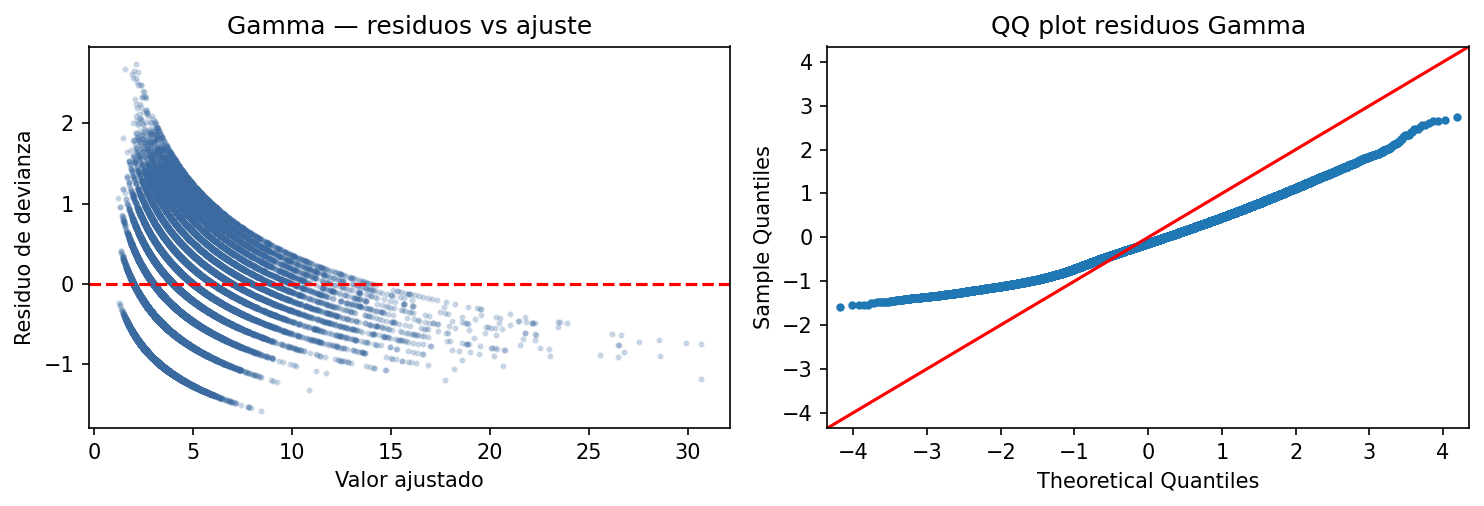
\includegraphics[width=0.95\linewidth]{figuras/fig5_diag_gamma.png}
\caption{Diagnóstico del modelo Gamma: residuos de devianza vs. valores ajustados (izquierda) y QQ plot (derecha).}
\label{fig:gamma}
\end{figure}

Los efectos multiplicativos más grandes vienen del número de procedimientos y de diagnósticos (cada unidad adicional multiplica la estancia esperada por $\approx 1.05$-$1.07$), y de algunas categorías diagnósticas: \textit{Neoplasmas} y \textit{Diabetes} como diagnóstico principal alargan la estancia un 24--29\% respecto a la categoría de referencia.

\subsection{¿Por qué no bosques aleatorios o XGBoost?}
Pregunta inevitable. La respuesta corta es: interpretabilidad. Para un proyecto cuya audiencia final es la directiva médica, poder decir ``cada ingreso previo multiplica las odds por 1.40'' es infinitamente más útil que un feature-importance ordinal. Hicimos una prueba rápida con \texttt{RandomForestClassifier} de default y el AUC subió apenas a 0.635 --- mejora marginal que no compensa la pérdida de lectura clínica. Además, los tres modelos elegidos (logística, binomial negativa, Gamma) comparten la estructura GLM y son los que el currículo de la materia sugiere como herramientas primarias \cite{mccullagh1989}.

\section{Conclusiones y Recomendaciones}
Tres ideas para llevarle a la directiva, ordenadas de más a menos accionables:

\textbf{Primera: un programa de transición de cuidados enfocado.} El predictor modificable más fuerte de readmisión a 30 días es el patrón previo de utilización --- ingresos recientes y visitas a urgencias. Un piloto que identifique a este subgrupo al alta y les agende llamada de seguimiento a 72 horas más cita ambulatoria a 7 días atacaría justamente la palanca que el modelo señala. Literatura reciente sugiere reducciones de readmisión del 15--25\% con intervenciones así \cite{jencks2009}.

\textbf{Segunda: el vector \textit{especialidad desconocida}.} Los pacientes cuya especialidad responsable quedó sin registrar tienen el doble de tasa de ingresos. Antes de quedarnos con la explicación clínica, habría que investigar si es un tema de captura de datos --- quizás son pacientes de urgencias que no pasaron a ninguna especialidad. La recomendación práctica es auditar el flujo de registro, no cambiar nada clínicamente.

\textbf{Tercera: planeación de camas por perfil diagnóstico.} El modelo Gamma sugiere que los casos de neoplasmas y complicaciones diabéticas duran un 25--30\% más. Incorporar este factor al modelo de planeación de ocupación ayudaría a reducir cuellos de botella durante los picos estacionales.

\subsection*{Limitaciones}
El AUC modesto (0.608) es la limitación más honesta que podemos reportar. El dataset no trae valores detallados de HbA1c ni resultados de laboratorio puntuales, y sin esos biomarcadores fundamentales ningún modelo va a alcanzar los AUC $> 0.75$ que sí logra la literatura con datos enriquecidos. En un siguiente paso valdría la pena fusionar este dataset con notas clínicas vía embeddings de texto --- pero eso ya es otro proyecto.

Otra limitación importante: quedarnos sólo con el primer encuentro por paciente es conservador pero nos costó casi una tercera parte de los datos. Un abordaje alternativo sería un modelo mixto con efectos aleatorios a nivel de paciente (\texttt{GEE} o \texttt{mixedlm} en statsmodels), que permitiría aprovechar todas las admisiones respetando la estructura de correlación intra-sujeto. Lo dejamos marcado como mejora futura porque excede el alcance de esta materia.

Finalmente, la base de datos corresponde a 1999--2008 en hospitales estadounidenses. Las prácticas clínicas y los protocolos de alta de diabetes han cambiado desde entonces, así que las conclusiones específicas son orientativas más que prescriptivas. La metodología, en cambio, sí es transferible a datos más recientes de hospitales mexicanos, que sería el siguiente paso natural.

\begin{thebibliography}{00}
\bibitem{strack2014} B. Strack, J. P. DeShazo, C. Gennings, et al., ``Impact of HbA1c measurement on hospital readmission rates,'' \textit{BioMed Research International}, vol. 2014, 2014. Recuperado de: \url{https://doi.org/10.1155/2014/781670}
\bibitem{cms_hrrp} Centers for Medicare \& Medicaid Services, ``Hospital Readmissions Reduction Program (HRRP),'' 2024. Recuperado de: \url{https://www.cms.gov/medicare/payment/prospective-payment-systems/acute-inpatient-pps/hospital-readmissions-reduction-program-hrrp}
\bibitem{ahrq_ccs} Agency for Healthcare Research and Quality, ``Clinical Classifications Software (CCS) for ICD-9-CM,'' 2023. Recuperado de: \url{https://hcup-us.ahrq.gov/toolssoftware/ccs/ccs.jsp}
\bibitem{rubin2018} D. J. Rubin, ``Hospital readmission of patients with diabetes,'' \textit{Current Diabetes Reports}, vol. 15, no. 4, 2015. Recuperado de: \url{https://doi.org/10.1007/s11892-015-0584-7}
\bibitem{jencks2009} S. F. Jencks, M. V. Williams, and E. A. Coleman, ``Rehospitalizations among patients in the Medicare fee-for-service program,'' \textit{New England Journal of Medicine}, vol. 360, no. 14, pp. 1418--1428, 2009. Recuperado de: \url{https://doi.org/10.1056/NEJMsa0803563}
\bibitem{statsmodels} S. Seabold and J. Perktold, ``statsmodels: Econometric and statistical modeling with Python,'' 2024. Recuperado de: \url{https://www.statsmodels.org/stable/index.html}
\bibitem{cameron2013} A. C. Cameron and P. K. Trivedi, ``Regression Analysis of Count Data,'' 2nd ed., Cambridge University Press, 2013. Resumen recuperado de: \url{https://cameron.econ.ucdavis.edu/racd2/}
\bibitem{scipydocs} P. Virtanen et al., ``SciPy 1.0: fundamental algorithms for scientific computing in Python,'' \textit{Nature Methods}, vol. 17, pp. 261--272, 2020. Recuperado de: \url{https://doi.org/10.1038/s41592-019-0686-2}
\bibitem{mccullagh1989} P. McCullagh and J. A. Nelder, ``Generalized Linear Models,'' 2nd ed., Chapman \& Hall/CRC, 1989. Descripción recuperada de: \url{https://www.routledge.com/Generalized-Linear-Models/McCullagh-Nelder/p/book/9780412317606}
\end{thebibliography}

\end{document}
